\documentclass{beamer}
\usetheme{Rochester}

\input{/home/dhanus/Documents/latex-headers/header_presentation.tex}
\title{A Greedy Path-Based Algorithm for Traffic Assignment}
\author{Jun Xie, Yu Nie, Xiaobo Liu}
\date{\today}

\begin{document}

\begin{frame}
    \titlepage
\end{frame}

\begin{frame}{Introduction}
\begin{itemize}
    \item The UE-TAP has been used as a standard tool to
    predict network flows.

    \item Path based algorithms solve this problem by storing
    a set of paths for each O-D pair, which are iteratively
    generated by `column generation'.

    \item Limitations: 
    \begin{itemize}
    \item storing and manipulating paths
    require a lot of memory
    \item decomposing scheme by O-D pairs
    generate a large number of sub-problems.
    \end{itemize}

\pause

    \item RAM capacity no longer an issue!

    \item Path based algorithms are easier to understand and
    implement, compared to many other methods.
\end{itemize}
\end{frame}

\begin{frame}{Overview}
The paper presents a new path-based algorithm for the
UE-TAP, which is more efficient than most modern algorithms.

\pause

\begin{enumerate}
\setcounter{enumi}{-1}
    \item Introduction
    \item Theory
    \item Algorithm
    \item Results
\end{enumerate}
\end{frame}

\begin{frame}{Setup and Notation}
\begin{itemize}
    \item $G(N,A)$ -- strongly connected directed transportation network.
    $N$ set of nodes, $A$ set of links.

    \item $R, S\subseteq N$, collection of origin and destination nodes.

    \item $d_{rs}$, the travel demand between $r\in R$ and $s\in S$.

    \item $H_{rs}$ -- set of simple paths between $r$ and $s$.

    \item $(i,j)$ -- link with head node $i$ and tail node $j$.
    $t_{ij}(x_{ij})$ is the cost of traversing $(i,j)$. The
    function $t_{ij}(\cdot)$ is strictly positive and monotonically
    increasing.

    \item For path $h\in H_{rs}$, the flow in $h$ will be
    denoted by $f_h$.
\end{itemize}
\end{frame}

\begin{frame}{Wardrop's Principle}
\begin{definition}[UE-Condition]
    For each O-D pair $(r,s)$, every used path between $r$ and
    $s$ must have equal and minimal travel-time.
\end{definition}

This can be formulated as an optimization problem.

\[
    \min z(f) = \sum_{(i,j)\in A} \int_0^{
    x_{ij}
    } t(\omega)d\omega
\]
where
\[
    x_{ij} = \sum_{r\in R}\sum_{s\in S}\sum_{h\in H_{rs}}f_h
    \delta_{ij}^h
\]
Subject to:
\[
\begin{split}
    f_h\geq 0 \text{ and }\sum_{h\in H_{rs}} f_h = d_{rs}\quad \forall\, r\in R,s\in S
\end{split}
\]
\end{frame}

\begin{frame}{Approximation}
\begin{itemize}
    \item Solution to the above problem satisfies
    UE-condition.
    
    \item Will use quadratic approximation of the
    Beckman function as the objective function.

    \item Consider the case of a single O-D pair.

    \item Second order Taylor approximation at path flow
    solution $g$:
    \[
        \hat{z}_{rs}(f) \approx z_{rs}(g) +
        \sum_{h\in H_{rs}}\frac{\partial z_{rs}}{\partial f_h}\bigg|_{g}
        (f_h-g_h)+
        \sum_{h\in H_{rs}} \frac{\partial ^2 z_{rs}}{\partial f_h^2}\bigg|_g(f_h-g_h)^2
    \]

    \item Denote $\frac{\partial z_{rs}}{\partial f_h}\big|_{g}=: v_h^g$ and
    $\frac{\partial ^2 z_{rs}}{\partial f_h^2}\big|_g =: s_h^g$.

    \item After removing constants, objective becomes:
    \[
        \sum_{h\in H_{rs}}\big[(v_h^g - s_h^g g_h)f_h + \frac{1}{2}
        s_h^g f_h^2\big]
    \]
\end{itemize}
\end{frame}

\begin{frame}{KKT Conditions}
These constants can be calculated easily by
taking the derivative of the Beckman function.

\[
\frac{\partial z_{rs}}{\partial f_h}\bigg|_{g}
= \sum_{(i,j)\in A}\delta_{ij}^h t_{ij}(x_{ij});\quad
\frac{\partial ^2 z_{rs}}{\partial f_h^2}\bigg|_g
= \sum_{(i,j)\in A} \delta_{ij}^h t'_{ij}(x_{ij})
\]

The KKT conditions of the modified problem with the
same constraints as before imply:

\[v_h^g + s_h^g(f_h-g_h) - w_{rs} \geq 0\]
and 
\[f_h(v_h^g + s_h^g(f_h-g_h) - w_{rs}) = 0\]

Here the Lagrange multiplier (for the equality constraint),
$w_{rs}$ is interpreted as the least travel cost between
$r$ and $s$.


\end{frame}

\begin{frame}{More Notations}
Note that
\[
\hat{v}_h = v_h^g + s_h^g(f_h-g_h)
\]
is a first order approximation of the path travel cost.

Put
\[
c_h^g := v_h^g - s_h^g g_h
\]
then the conditions seen in previous slide for used paths
($\hat{H}_{rs}$) become
\[
    c_h^g + s_h^g f_h = w_{rs} := \bar{w}_{rs} \quad \forall h\in\hat{H}_{rs}
\]
\end{frame}


\begin{frame}{Path Flow Updates}
Dividing the above expression by $s_h^g$ and summing over
all paths,
\[
    \bar{w}_{rs} = \frac{d_{rs} + \sum_{h\in \hat{H}_{rs}}
    ({c_h^g}/{s_h^g})}{\sum_{h\in\hat{H}_{rs}}{1}/{s_h^g}}
\]

And the new flows are
\[
    f_h = \frac{\bar{w}_{rs}-c_h^g}{s^g_h}
\]

The paths in $H_{rs}\setminus \hat{H}_{rs}$ recieve
zero flow.
\end{frame}


\begin{frame}{Algorithm -- Single O-D Pair}
Takes some initial path flow vector $\{g_h: h\in H_{rs}\}$
as input and outputs updated path flow vector.
The steps involved are:
\begin{enumerate}
    \item Calculate the constants $v_h^g, s_h^g$ and
    $c_h^g$.

    \item Sort paths based on increasing $c_h^g$.

    \item Add the path with smallest $c_h^g$ to $\hat{H}_{rs}$
    and update $\bar{w}_{rs}$.

    \item Keep adding subsequent paths until $c_h^g$ exceeds
    $\bar{w}_{rs}$.

    \item Update the flows.

    \item The new path flow vector $\hat{H}_{rs}$ is given as
    output.
\end{enumerate}
\end{frame}


\begin{frame}{Algorithm -- Single O-D Pair}
\begin{columns}
    \begin{column}{0.4\textwidth}
    \begin{figure}
    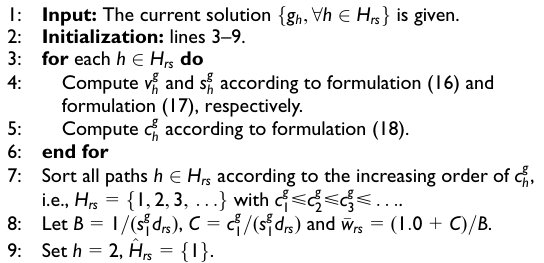
\includegraphics[width=\textwidth]{./alg11.jpg}
    \end{figure}
    \end{column}

    \begin{column}{0.2\textwidth}
    \begin{figure}
    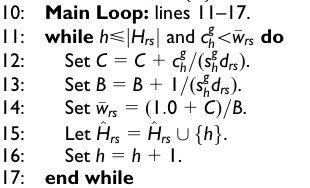
\includegraphics[width=\textwidth]{./alg12.jpg}
    \end{figure}
    \end{column}

    \begin{column}{0.4\textwidth}
    \begin{figure}
    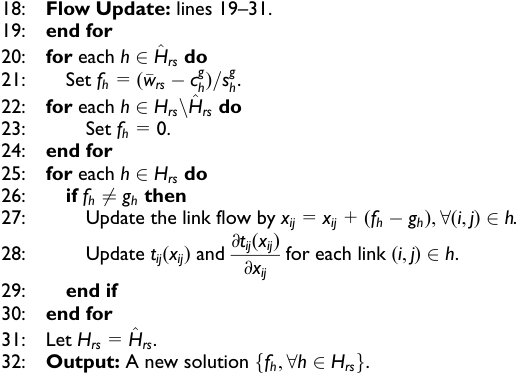
\includegraphics[width=\textwidth]{./alg13.jpg}
    \end{figure}
    \end{column}
\end{columns}
\end{frame}


\begin{frame}{Initialization}
    \begin{figure}
    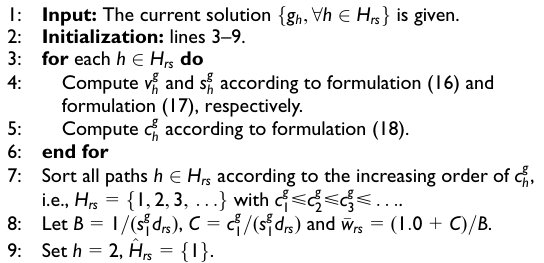
\includegraphics[width=\textwidth]{./alg11.jpg}
    \end{figure}
\end{frame}


\begin{frame}{Main Loop}
    \begin{figure}
    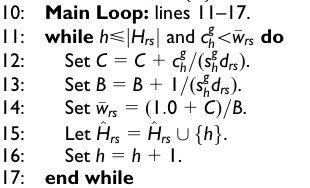
\includegraphics[scale=0.5]{./alg12.jpg}
    \end{figure}
\end{frame}


\begin{frame}{Flow Update}
    \begin{figure}
    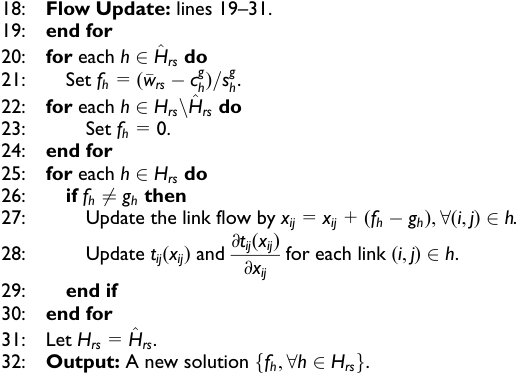
\includegraphics[width=\textwidth]{./alg13.jpg}
    \end{figure}
\end{frame}

\begin{frame}{Greedy Path-Based Algorithm}
The steps involved are:
\begin{enumerate}
\setcounter{enumi}{-1}
    \item Initialization: assign all passengers to shortest
    path between O-D pairs and set $H_{rs}$ to contain
    the shortest path between $r$ and $s$.

    \item Perform flow adjustment on $H_{rs}$ using the
    previous algorithm for each $r,s$.

    \item (Inner loop) Update flows on O-D pairs with larger deviation:
    \begin{itemize}
    \item If $\max{v_h} - \min{v_h}\geq RG^{k-1}/2$,
    for an O-D pair, $H_{rs}$ is passed to the previous
    algorithm again.

    \item If this update is not being done for any
    O-D pair (or if the iteration exceeds a limit),
    break from the loop.
    \end{itemize}

    \item Push the shortest path between each O-D pairs to
    $H_{rs}$ and repeat from step 1 until convergence.
\end{enumerate}
\end{frame}


\begin{frame}{Greedy Path-Based Algorithm}
\begin{columns}
    \begin{column}{0.33\textwidth}
    \begin{figure}
    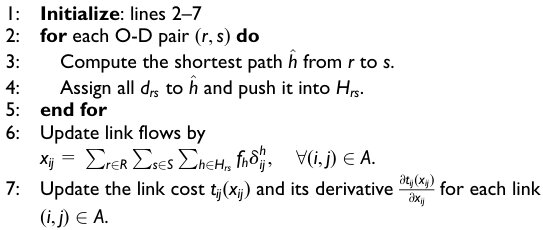
\includegraphics[width=\textwidth]{./alg21.jpg}
    \end{figure}
    \end{column}

    \begin{column}{0.33\textwidth}
    \begin{figure}
    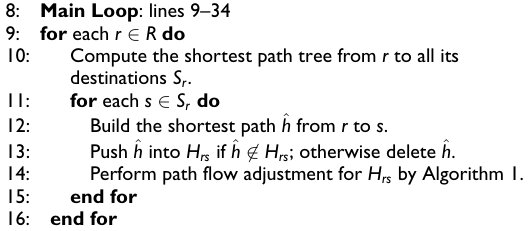
\includegraphics[width=\textwidth]{./alg22.jpg}
    \end{figure}
    \end{column}

    \begin{column}{0.33\textwidth}
    \begin{figure}
    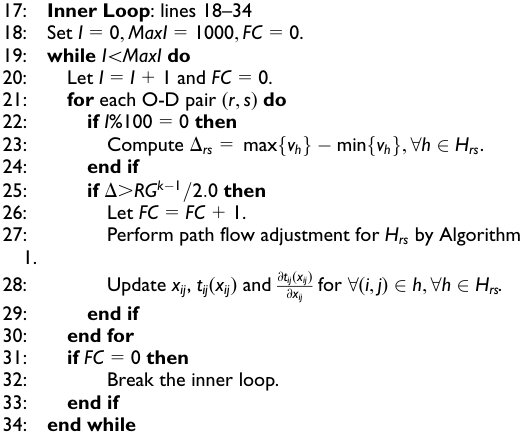
\includegraphics[width=\textwidth]{./alg23.jpg}
    \end{figure}
    \end{column}
\end{columns}
\end{frame}


\begin{frame}{Initialization}
    \begin{figure}
    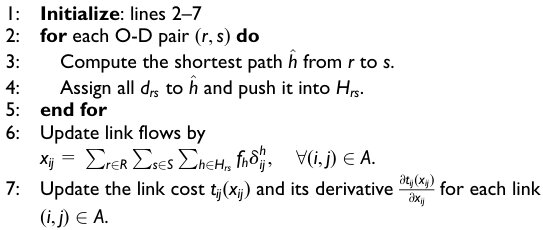
\includegraphics[width=\textwidth]{./alg21.jpg}
    \end{figure}
\end{frame}


\begin{frame}{Main Loop}
    \begin{figure}
    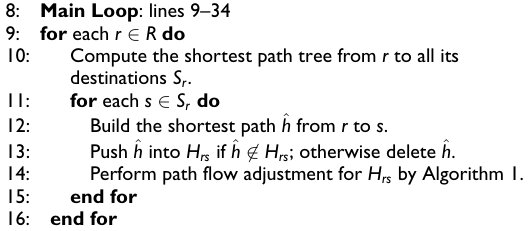
\includegraphics[width=\textwidth]{./alg22.jpg}
    \end{figure}
\end{frame}


\begin{frame}{Inner Loop}
    \begin{figure}
    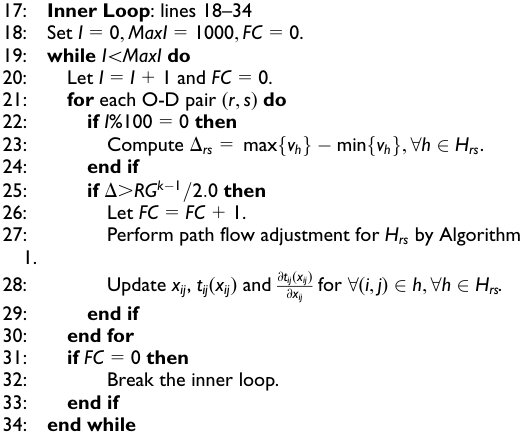
\includegraphics[scale=0.5]{./alg23.jpg}
    \end{figure}
\end{frame}



\begin{frame}{Results}
\begin{itemize}
    \item Numerical results were produced on Windows 10
    workstation with $3.3GHz$ Intel Xenon processor and
    $16 GB$ RAM using C++.

    \item The greedy algorithm performs better than GP, TAPAS,
    iTAPAS in all the experiments.

    \item iGP performs almost as good as the greedy method.
\end{itemize}
\end{frame}

\begin{frame}{Results}
\begin{figure}
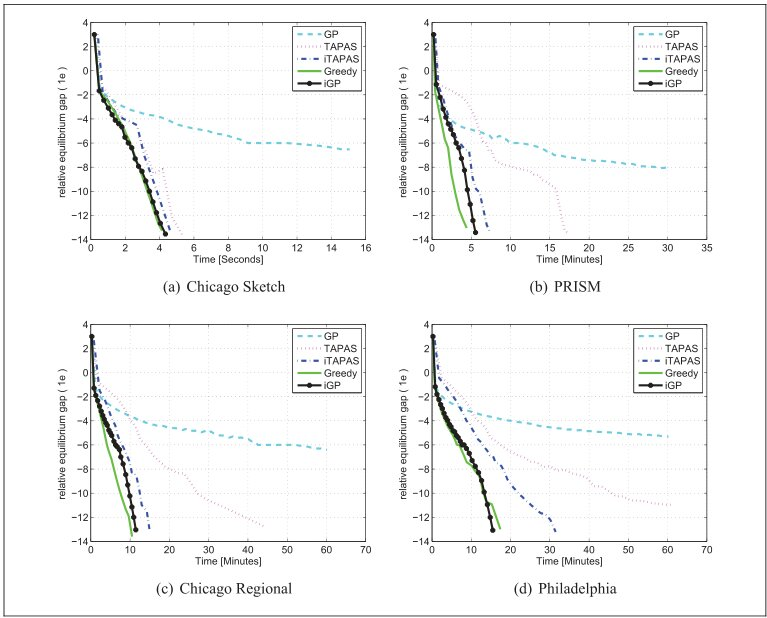
\includegraphics[scale=0.35]{./graph1.jpg}
\end{figure}
\end{frame}


\begin{frame}{Results}
Even without the inner loop, the greedy algorithm
performs better than GP.
\begin{figure}
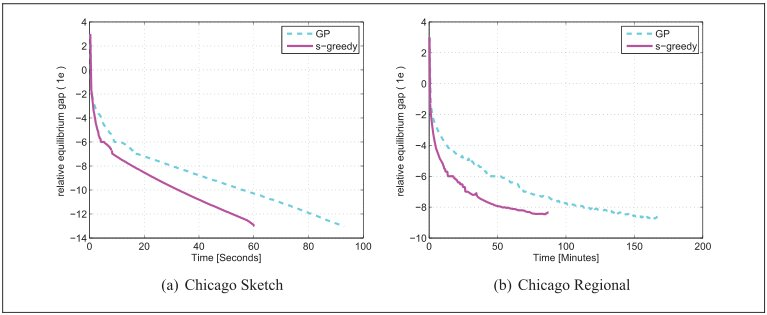
\includegraphics[width=\textwidth]{./graph2.jpg}
\end{figure}
\end{frame}


\begin{frame}{Results -- Memory Usage}
\begin{figure}
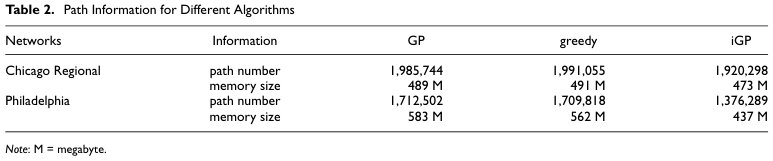
\includegraphics[width=\textwidth]{./table1.jpg}
\end{figure}

The path-based algorithms generates less than $2$ million
used paths, which consumes less than $600$ megabytes of
memory.
\end{frame}


\begin{frame}{Conclusion}
\begin{itemize}
    \item Frequency of path flow adjustments must be higher
    than that of column generation.

    \item More flow adjustment must be done on less converged
    O-D pairs.

    \item Do not try to get high precision results for
    sub-problems in the early iterations.
\end{itemize}
\end{frame}

\end{document}
